\newpage
\appendix
\section{Anhang}
\subsection{Schülerliste \& Graph}
\subsubsection*{Schülerliste}
\begin{figure}[H]
    \centering
    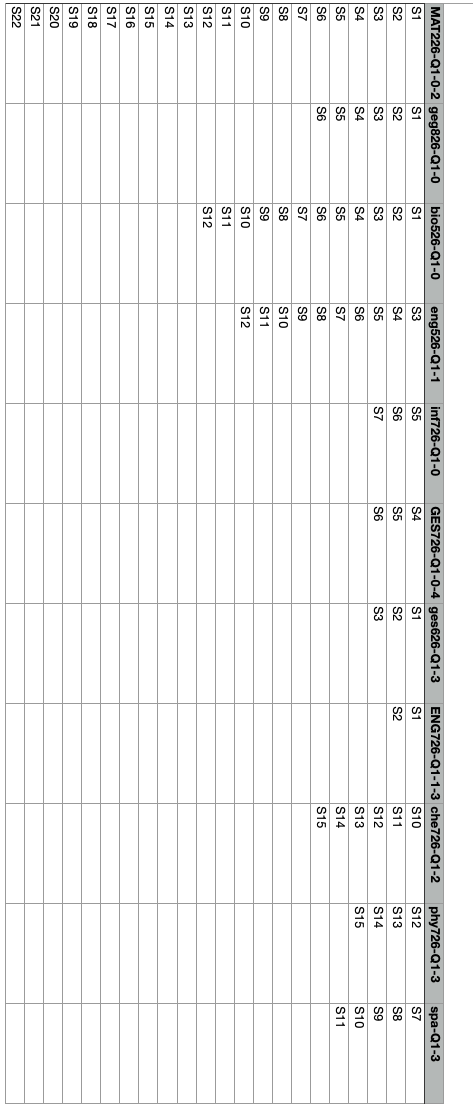
\includegraphics[width=0.5\linewidth]{docs/graphics/StudentList1.png}
    \caption{Schülerliste in Excel-Tabelle (anonymisierte Daten)}
    \label{fig:studenList}
\end{figure}
\begin{figure}[H]
    \centering
    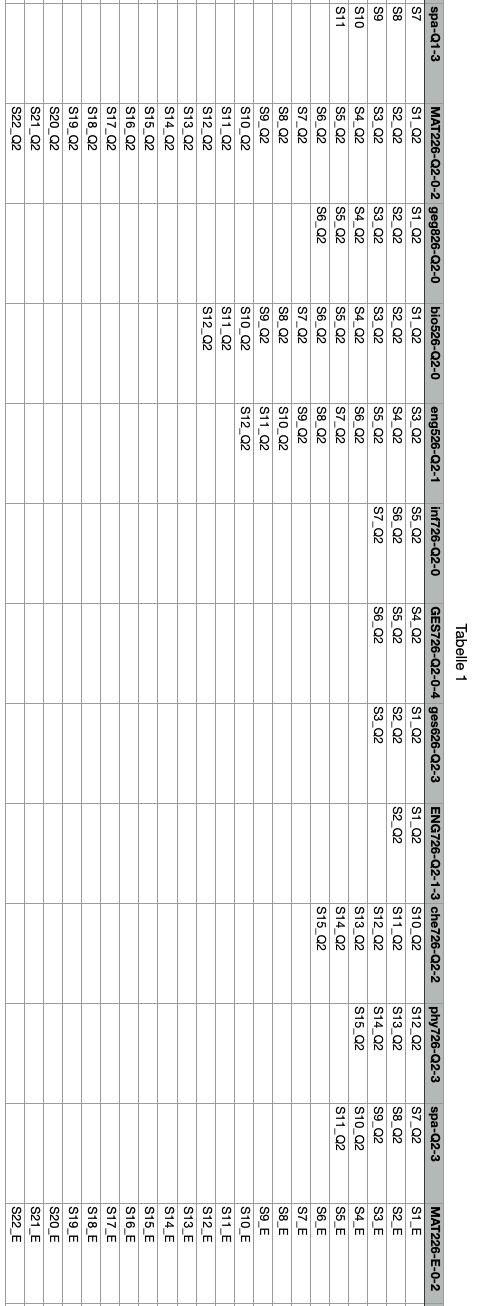
\includegraphics[width=0.6\linewidth]{docs/graphics/StudentList2.png}
\end{figure}
\begin{figure}[H]
    \centering
    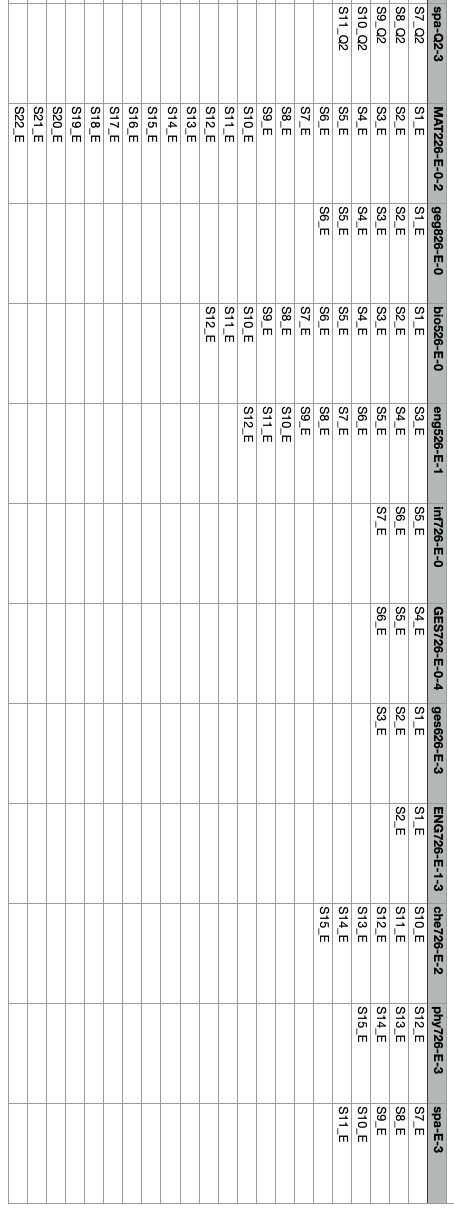
\includegraphics[width=0.6\linewidth]{docs/graphics/StudentList3.png}
\end{figure}

\newpage
\subsubsection*{Graph}
\begin{figure}[H]
    \centering
    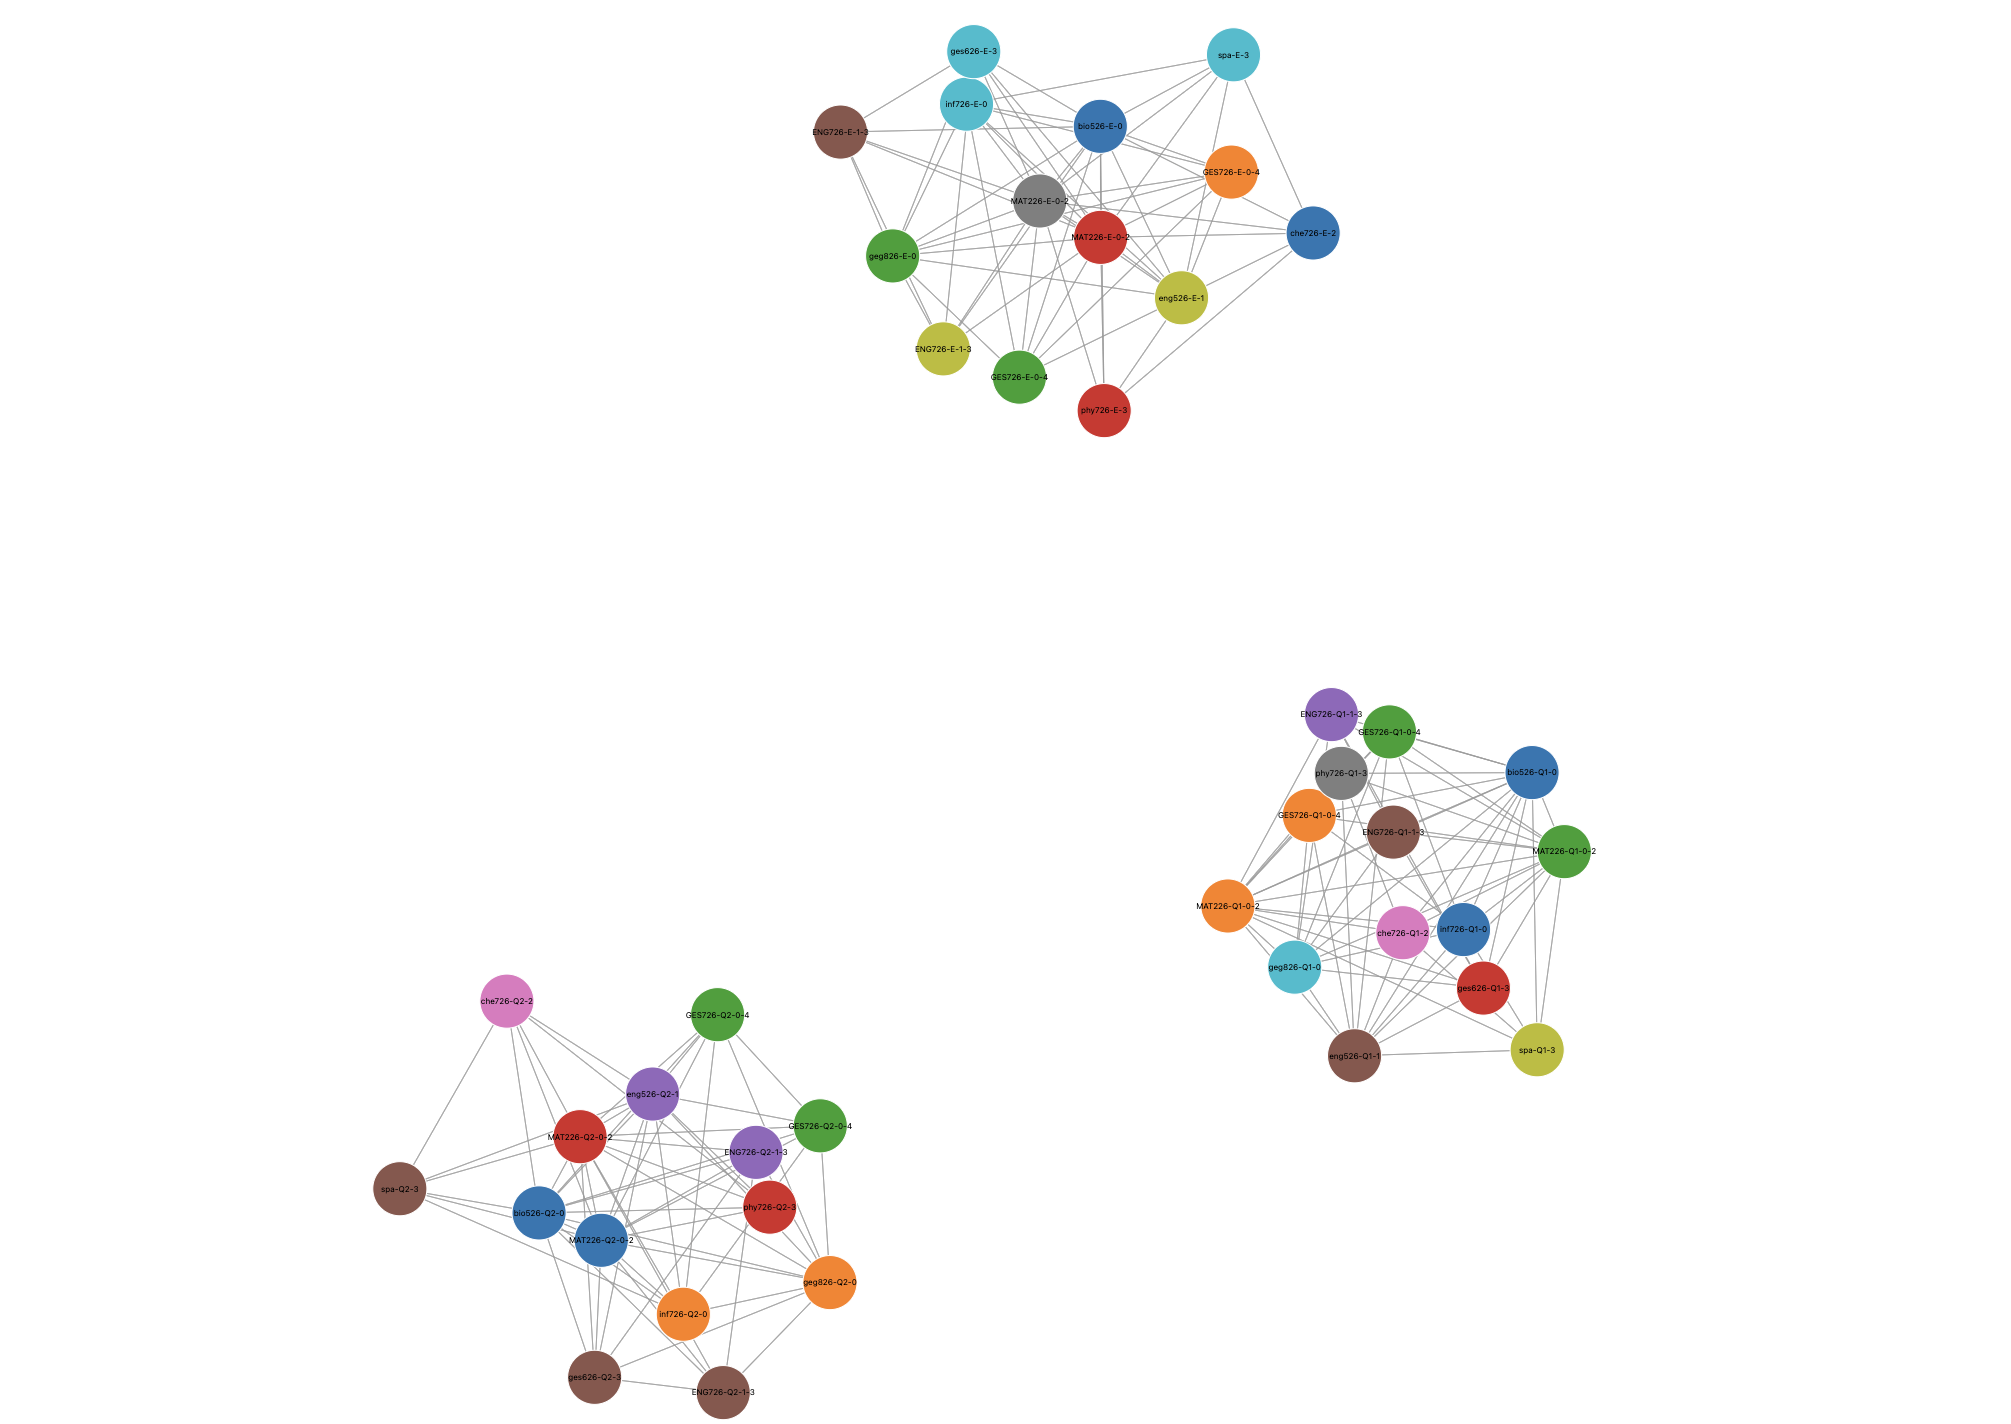
\includegraphics[width=0.5\linewidth]{docs/graphics/graph-all.png}
    \caption{Graph einer beispielhaften Implementierung}
    \label{fig:graph1}
\end{figure}
\begin{figure}[H]
    \centering
    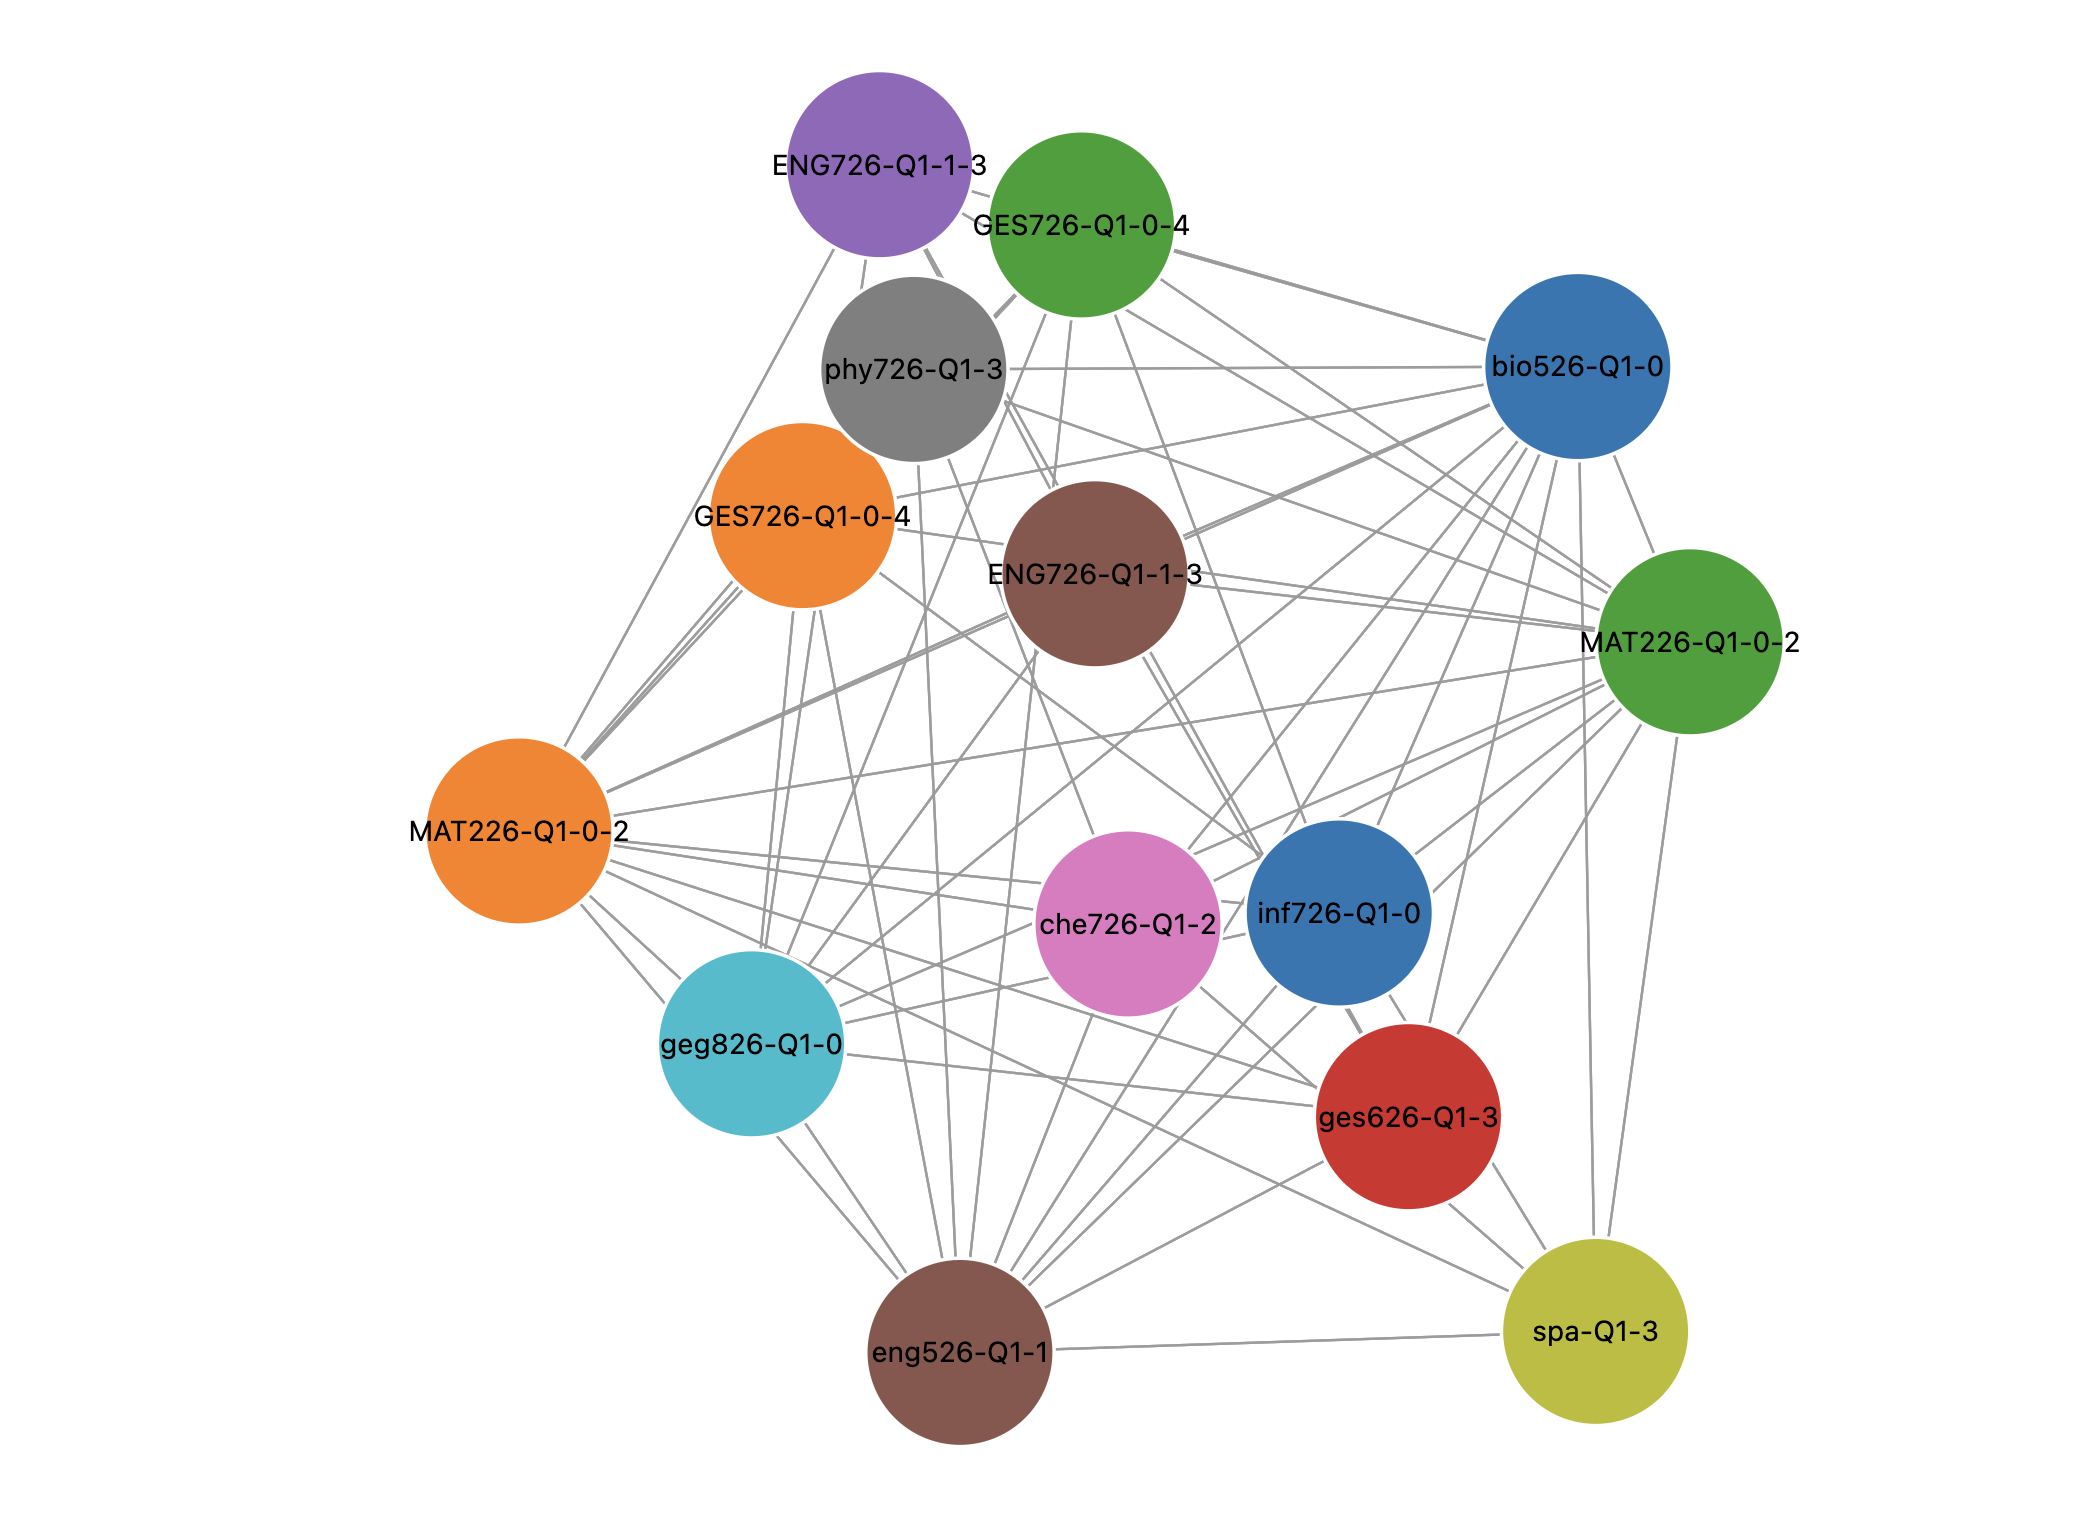
\includegraphics[width=0.5\linewidth]{docs/graphics/graph-detail.png}
    \caption{Teil des Graphen einer beispielhaften Implementierung}
    \label{fig:graph2}
\end{figure}
\begin{figure}[H]
    \centering
    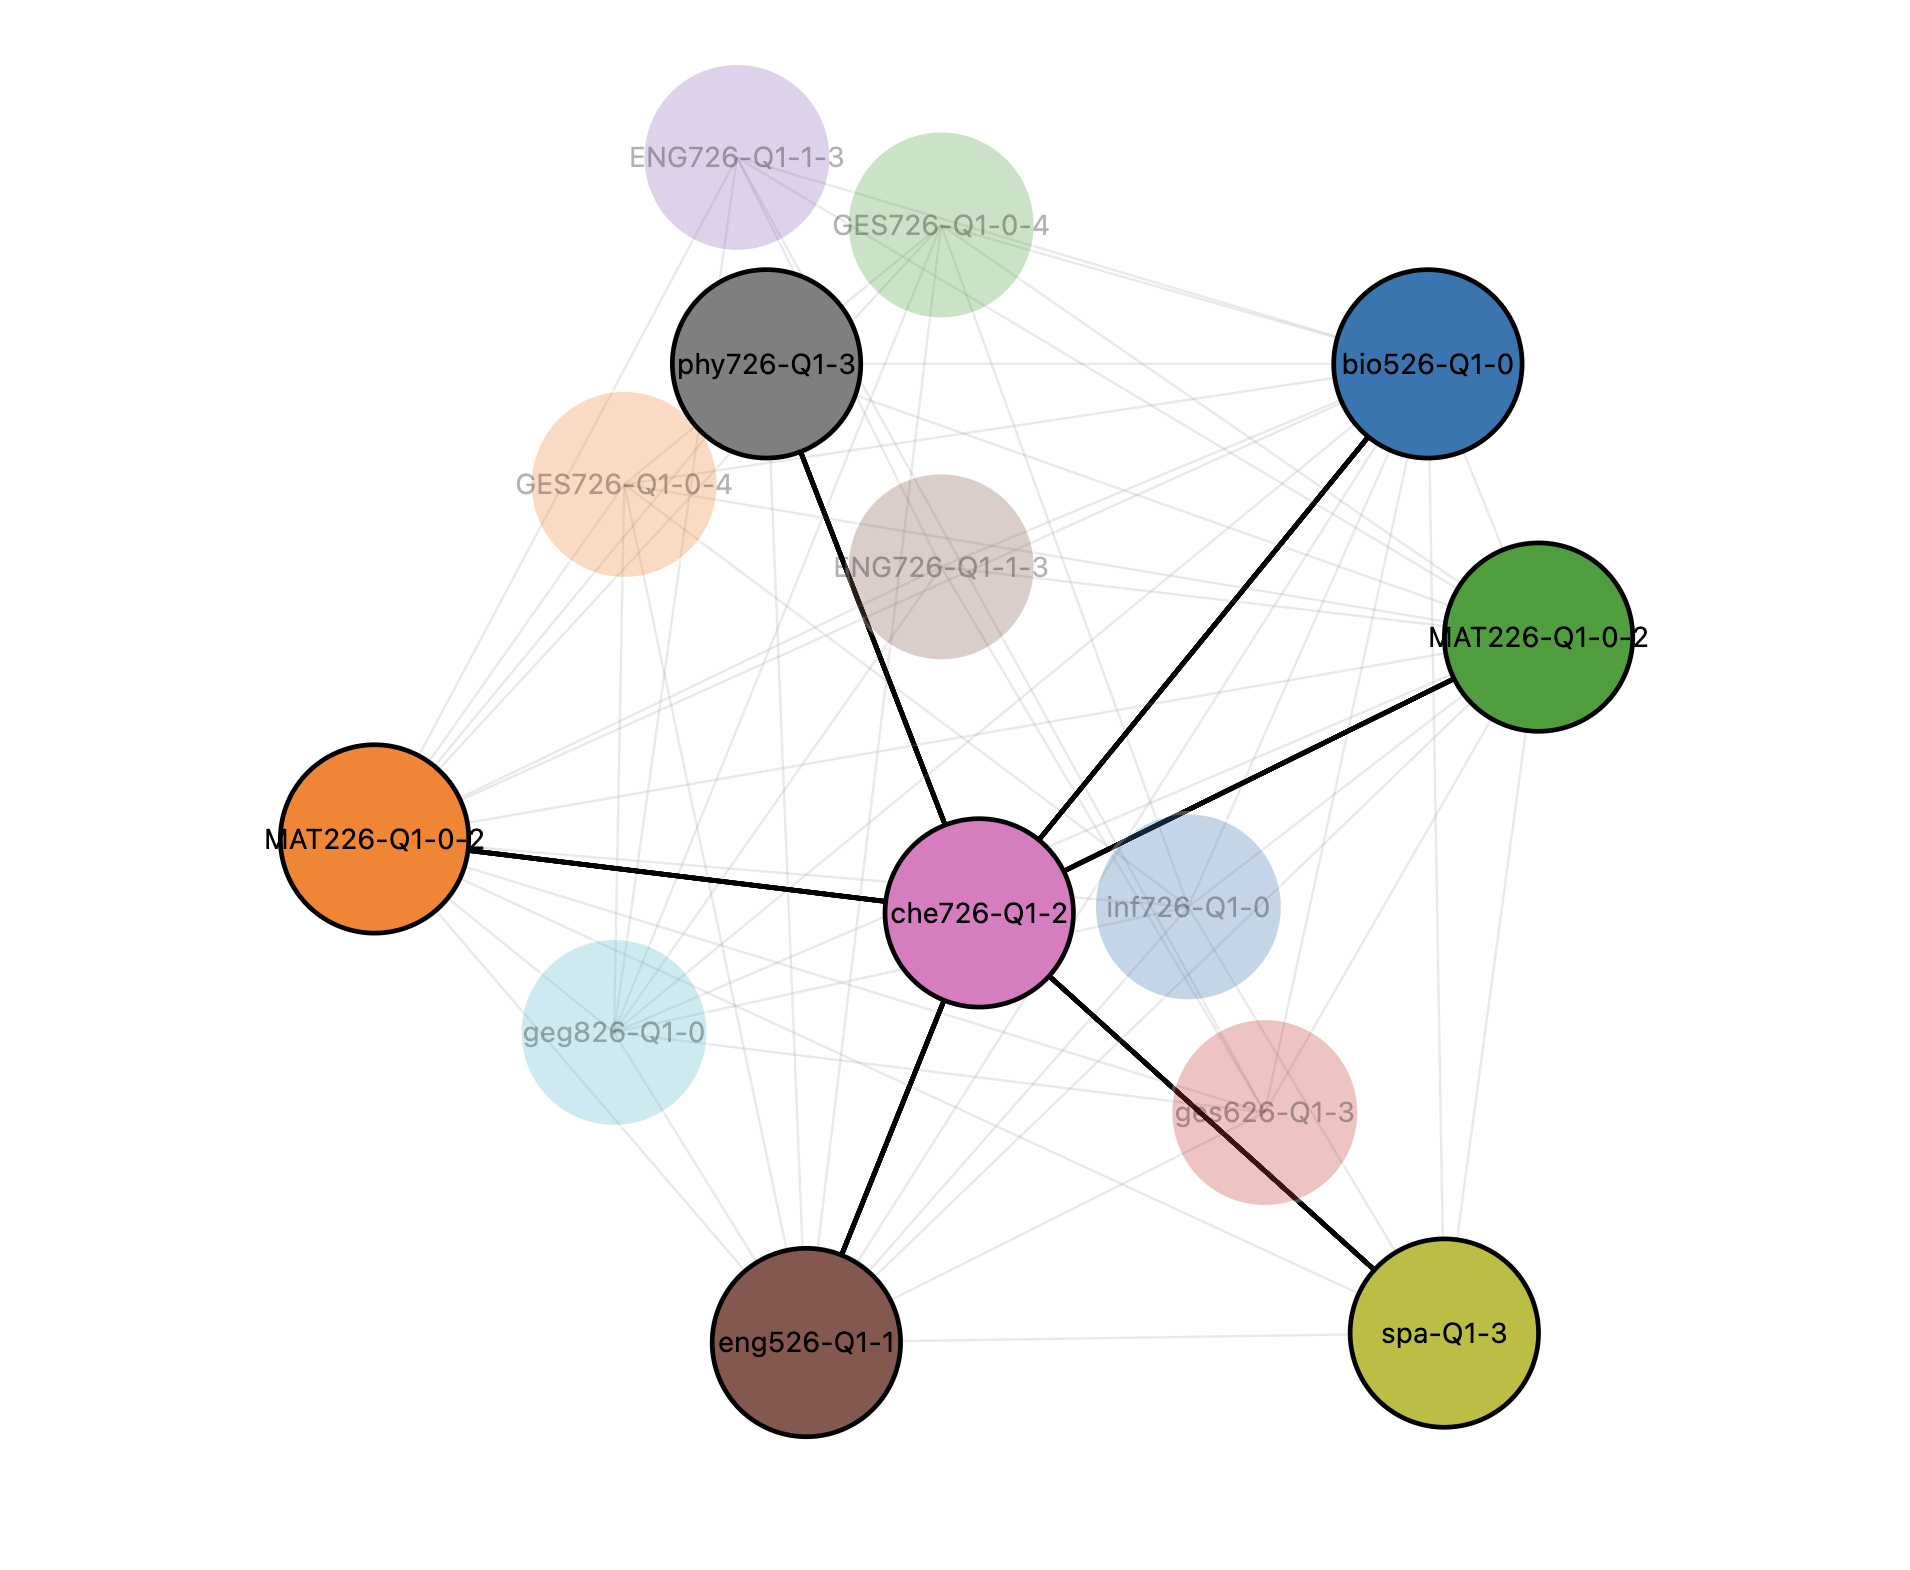
\includegraphics[width=0.5\linewidth]{docs/graphics/graph-detail-selected.png}
    \caption{Teil des Graphen einer beispielhaften Implementierung mit ausgewähltem Knoten}
    \label{fig:graph3}
\end{figure}


\newpage
\subsection{Klausurenplan}
\begin{figure}[H]
    \centering
    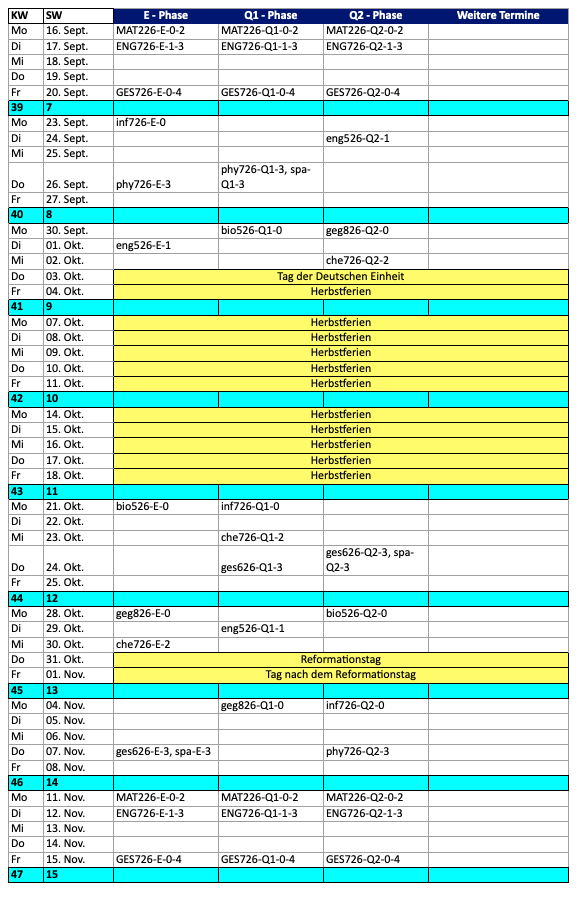
\includegraphics[width=0.8\linewidth]{docs/graphics/Klausurenplan.png}
    \caption{Klausurenplan als Excel-Tabelle}
    \label{fig:klausurenplan}
\end{figure}
Der 16. September ist der Montag, an dem die gewählte Klausurenphase beginnt. Dies ist nicht der Beginn des Schuljahres.